\chapter{Introduction}
\label{Introduction}
Phages are small viruses, measuring 27-190 nm in diameter, that infect and lyse (kill) specific bacteria. 
Phages act as nature's antimicrobial defense, but they also impact bacterial evolution and resource turnover. 
There are various medical and industrial applications for phages to control bacterial growth; however, to realize these applications, it is essential to understand how phages interact with bacteria, enabling the implementation of a robust method to control bacterial growth. 

\section{Thesis Overview}
To answer the question of how phages, bacteria, resources, and their interactions can be mathematically modeled, I developed a simulation framework that can model and interact with any $p\times b\times r$ system, where $p$ represents the number of phages, $b$ represents the number of bacteria and $r$ represents the number of resources. 
Using the software, I answer how phages impact community dynamics in complex microbial communities. 

First, there is a biological introduction to phages and bacteria. 
This introduction covers how phages infect bacteria, how bacteria defend against phages, how phages defeat bacterial defenses, and how phages defend against other phages. 
There is an introduction to different methods of modeling phage and bacteria dynamics. 
This thesis provides a brief overview of software that models phages, resources, bacteria, and their associated limitations. 
This thesis presents software I developed to support the research, demonstrating its capabilities using a representative model of phage, bacteria, and resource interactions. 
The section also provides an overview of its usage, including example outputs from demonstration runs.
I use the software to analyze various scenarios, such as phage proliferation under a washout scenario, and analyze growth rate-limited regions. 

\section{The Environment}
In ecosystems like the ocean, the gut, or soil, there are thousands of different microbes that interact with one another or with their surrounding environment.
The interactions are complex, with many factors affecting the growth of bacteria and phages. 
The interactions between entities in the environment are often synergistic. 
When an animal dies, bacteria begin to digest and decompose the animal into simpler chemicals, such as carbon and nitrogen, which plants can use to grow. 
Animals then eat these plants, and the cycle continues. 
External factors, such as flooding, droughts, chemical spills, or the introduction of new entities, have a massive impact on the ecosystem. 
These events can add or remove resources from the system, alter environmental parameters such as the temperature and acidity of the soil, introduce competition, or create a population imbalance by killing microorganisms. 
These effects have a larger effect on the ecosystem and food chain as a whole, as bacteria are one of the fundamental foundations for resource recycling. 

\section{Biological Background}
Phages are small viruses on the order of 27-190 nm (the average size of marine phages is 54 nm) that infect and lyse (kill) specific bacteria.
The phage cycle process starts with a phage coming into contact with a bacterium \Cref{fig:cyanobacteria_bloom_cycle}.
Once it has identified an injection site, the phage can inject a strain of DNA into the bacteria.
The DNA strand has two options. 

The first option is that the phage can enter the lysogenic cycle by integrating its DNA into the host cell's DNA. 
Prophages are phages that have integrated with the host cell's DNA. 
The new cell will contain the prophage's DNA as the bacteria replicate. 
The phage will exit the lysogenic cycle and enter the lytic cycle after receiving a signal, such as cell damage, and hijack the DNA replication mechanism. 

The second option is that the phage immediately enters the lytic cycle by hijacking the DNA replication process to create copies of its DNA. 
The phage will create multiple copies of itself using the host's transcription and translation machinery to replicate itself.
The phages self-assemble inside the bacteria until they lyse the cell (e.g., through chemically induced rupture of the cell wall), releasing the phages into the environment. 

\begin{figure}
    \centering
    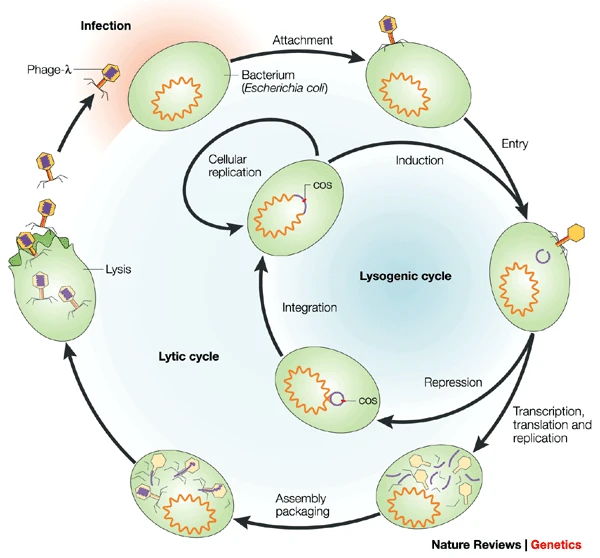
\includegraphics[width=0.5\linewidth]{Figures/phage_life_cycle.png}
    \caption{Life cycle of a phage, inside and outside a bacteria cell. Significant steps in the life cycle of a phage include the infection stage, integration, replication, and lysing process. Figure sourced from \citet{campbellFutureBacteriophageBiology2003}. }
    \label{fig:phage_life_cycle}
\end{figure}

\subsection{Phage's Role in the Environment}
Phages play a significant role in the ecosystem. 
Phage-mediated death occurs when phages infect susceptible bacteria, resulting in cell lysis and the release of cellular contents and nutrients that other organisms, such as bacteria and plants, can utilize. 
This process not only reduces bacterial populations but also accelerates the turnover of resources, such as nitrogen and carbon, for other bacteria and plants to utilize. 
Phages also help mediate horizontal gene transfer, disperse pathogenic diseases, and spread antibiotic resistance \cite{al-shayebCladesHugePhages2020}. 
Phages directly alter bacteria population diversity and population fitness by introducing new ways for bacteria to mutate \cite{brownEcologicalFunctionalRoles2022}. 

There are about $10^6$ bacteria cells/ml and $10^7$ phages/ml of marine water. 
About 5\% of any bacteria are currently infected, and phages account for about 15\% of daily bacterial deaths \cite{chibani-chennoufiPhageHostInteractionEcological2004}. 
Phage populations grow by infecting their hosts, but they can also be degraded, e.g., by UV radiation. 
UV is a significant factor in deactivating marine phages, causing up to a 5\% reduction in phage infectivity per hour \cite{chibani-chennoufiPhageHostInteractionEcological2004}. 

\subsubsection{Phages and Controlling Bacterial Blooms}
\textit{Cyanobacteria} cause damage to aquatic life by consuming resources and oxygen, starving aquatic life, and negatively affecting human health. 
Scientists are investigating the potential use of phages to control cyanobacteria (also known as blue-green algae) blooms in the environment \cite{colomaFrequencyVirusresistantHosts2019}. 
There is hope that phages can biologically control water quality in wastewater treatment plants and in the environment without the use of harsh chemical processes that would otherwise pose environmental and health hazards \cite{krysiak-baltynSimulationPhageDynamics2017, tuckerIdentificationCyanophageMaLBP2005}. 
\Cref{sec:AppendixB:environmental_protection} contains more information about controlling \textit{Cyanobacteria}. 

\section{Phage Cocktails and Human Health}
There is particular interest in phage applications in human and animal health, called phage therapy. 
There are approximately 100 trillion microbes, comprising about 5,000 different types of bacterial strains, in the human gut. 
The phages will target the specific bacteria of interest, for example, \textit{E. coli}, but they will not affect the other bacteria found in the human gut. 
Antibiotics indiscriminately affect any bacteria, disrupting the intricate ecosystem of the gut microbiome, acting as a scorched-earth mechanism. 
Antibiotics have also faced the challenge that bacteria are growing resistant to them, making the antibiotics less effective in the future \cite{odonkorBacteriaResistanceAntibiotics2011, volkovaEffectsEarlylifePenicillin2021}. 

Phages, on the other hand, specifically target a specific bacterial strain. 
Antibiotic-resistant bacteria are typically less resistant to phages. 
The bacteria cell typically has a trade-off between antibiotic resistance and phage resistance. 
So by designing phages to be highly infective, there is hope that the phage-resistant bacteria will lose the antibiotic resistance to counter the phages \cite{laurePhageResistancemediatedTradeoffs2022, zhaoPhagedrivenCoevolutionReveals2024}. 
\Cref{sec:AppendixB:phage_therapy_and_antibiotics} offers a more in-depth look at how healthcare professionals can utilize phages.

\section{Potential Applications of Phages}
Phages have numerous applications in industrial settings. 
Phage therapies can prevent the spread of common bacteria in livestock by incorporating phage therapy into the animal feed. 
Farmers often raise livestock in cramped spaces with inadequate sanitation facilities, which increases the risk of disease spreading. 
Factories can utilize phages to control the growth of bacteria, such as \textit{Salmonella} while producing food \cite{sofferBacteriophagesSafelyReduce2016, kowalskaFreshVegetablesFruit2023}. 
\Cref{sec:AppendixB:controlling_foodborne_bacteria} in \Cref{AppendixB} goes into more detail about using phages to control foodborne bacteria. 

\section{Modelling Phages in a Complex Community}
What we know about phages mechanistically often comes from well-researched bacteria in a laboratory, such as \textit{E. coli} and its phages, and what we know about phages in the environment comes from metagenomic surveys. 
Making the connection between the mechanistic and metagenomic models, which would enable us to develop and test different models, is the challenging part. 
Because of this, we need mathematical models to help bridge the gap between the lab and the environment. 
There have been previous attempts to model the complex dynamics of populations between phages, bacteria, and resources within the environment using Ordinary Differential Equations (ODEs) and Delay Differential Equations (DDEs).
Researchers cannot identify every interaction in the complex community, and even if they identify an interaction, they must experimentally derive the associated parameter values. 

There are two primary methods for modeling phage-bacteria dynamics: spatial and non-spatial.
In a spatial model, phages and bacteria can move through space and interact with their neighbors. 
Researchers have used partial differential equations (PDE) and cellular agent-based models (ABM) to model spatial interactions.
Spatial models lead to more computationally complex models but can result in more biologically realistic results. 
By contrast, ODE and DDE models describe non-spatial models. 
In a non-spatial model, a well-mixed solution contains the bacteria and phages, and researchers make no distinctions regarding neighbors or distances to other entities. 
They simplify interactions with a probabilistic approach.
At time step $t$, a percentage $p$ of entities interact with each other.

Non-spatial models are easier to develop and understand and are more effective in modeling large populations, albeit at the cost of losing spatial information. 
For this thesis, the focus will be on modeling resource, phage, and bacteria interactions using an ODE model. 
I describe a phage-bacteria-resource system as a $ p\times b\times r$ system. 
Current modeling methods have mainly stayed with $1\times 1 \times 1$ models, meaning one phage, one bacteria, and one resource. 
This thesis aims to develop a simulation framework that can model any $p\times b \times r$ ODE system. 

\section{Software Overview}
The project contains three parts, with an optional fourth part.
The first section is to create the network interaction. 
Here, the user can define the number of resources, phages, and bacteria, who interacts with whom, and the strength and type of interactions. See \Cref{sec:network_creation_tool} for further information. 
In \Cref{sec:simulation_framework}, the user uploads the network model and parameters and, as output, receives the time data and population data as an array. 
\Cref{sec:visualization_framework} allows the user to interact with \Cref{sec:network_creation_tool} and \Cref{sec:simulation_framework} with a dashboard. 
The user can graphically edit the attribute values of the network's edges and nodes and run more advanced visualizations, such as changing a parameter value to observe its impact on the population count. 

Several plots are included out of the box, allowing the user to test them. 
The plots offered in Part 3 of the program provide interactivity, including the ability to hide and show lines and dots, zoom in and out, and hover over lines and dots to display more detailed data. 

Finally, the user can optionally run multiple simulations and download the data to their disk to create their own visualizations using \Cref{sec:custom_visualizations_and_framework}. 
The visualizations created in \Cref{sec:visualization_framework} can be recreated in \Cref{sec:custom_visualizations_and_framework}. 
The user can choose the same parameter values used for a specific plot in \Cref{sec:visualization_framework}, run the simulation (as described in \Cref{sec:ultimate_analysis}), download the data, and reimplement the graphs. 

The user can use the tool themselves by importing the Python classes in their code, initializing the classes, and passing the appropriate data. 